\documentclass{scrartcl}
\usepackage[utf8]{inputenc}
\usepackage{amsmath}
\usepackage{subcaption}
\usepackage{caption}
\usepackage{graphicx}
\usepackage[left=2cm, right=2cm, bottom=2.5cm, top=2.5cm]{geometry}

\title{MCMC Project}
\subtitle{Markov Chains and Algorithmic Applications}
\author{\textsc{Druță Gheorghe} \and \textsc{Mocanu Alexandru} \and \textsc{Sachtler Arne}}
\date{EPFL - December 2018}

\begin{document}
\maketitle

\section{Introduction}
The purpose of the project is to solve a problem of nonlinear estimation, which would imply an exponential time complexity if solved analytically. In order to avoid this exponential complexity, we tackle the problem by using a Markov Chain Monte Carlo (MCMC) approach to the problem.

\subsection{The problem}
We are given a feature matrix $\mathrm{W} = \{\mathrm{W}_{ij}\}$ of dimension $\mathrm{m} \times \mathrm{n}$ with its entries extracted i.i.d. from a normal distribution of mean 0 and variance 1. The objective is to recover the input vector $\mathrm{X} = (\mathrm{X_1}, ..., \mathrm{X_n})^T \in \mathrm{S} = \{-1, 1\}^n$ from the observations $\mathrm{Y} = (\mathrm{Y_1}, ..., \mathrm{Y_m})^T$, given by the following expressions:
\begin{equation}
Y_i = \varphi \left( \sum_{i=1}^m \frac{W_ij}{\sqrt{n}} X_j \right) = \varphi \left( \left[ \frac{WX}{\sqrt{n}} \right]_i \right), 1 \le i \le m
\end{equation}
where $\varphi$ represents the Rectified Linear Unit (ReLU) function acting component-wisely.
There is no clear way to find the exact solution to this problem, but to search the entire state-space. This is unfeasible when $\mathrm{n}$ gets large, as the state-space has size $2^\mathrm{n}$.

\subsection{The algorithm}
Having seen that if $\mathrm{n}$ increases, the estimation of $\mathrm{X}$ becomes unfeasible, we look for another approach, namely a Monte Carlo Markov Chain algorithm.
For this we first define an energy function as follows:
\begin{equation}
H_Y(x) = \sum_{i=1}^m \left| Y_i - \varphi \left( \left[ \frac{WX}{\sqrt{n}} \right]_i \right) \right|^2
\end{equation}
The aim is to minimize this energy using a Metropolis chain. We do the following steps:
\begin{enumerate}
    \item We initialize our estimation of $\mathrm{X}$ by a vector $\mathrm{x}^{(0)}$ for which we extract each coordinate uniformly at random from $\{-1, 1\}$.
    \item We use the base chain with the following transition process: at time step $\mathrm{t}$ we choose one of the coordinates $\mathrm{i}$ of the estimator vector $\mathrm{x}^{(t)}$ uniformly at random and flip the value obtaining the estimation of time step $\mathrm{t}+1$:
    \begin{equation}
        x^{(t+1)} = \left( x_1^{(t)}, ..., x_{i-1}^{(t)}, -x_i^{(t)}, ..., x_n^{(t)} \right)
    \end{equation}
    \item We accept the previous move with acceptance probability
    \begin{equation}
        a_{\beta}(x^{(t)}, x^{(t+1)}) = \min \left\{ 1, e^{-\beta \left( H_Y(x^{(t+1)}) - H_Y(x^{(t)}) \right)} \right\}
    \end{equation} where $\beta > 0$ is a hyperparameter called \textit{inverse temperature}.
    \item We repeat from step 2 until we reach a small enough energy.
\end{enumerate}
In addition to the mentioned steps of the algorithm, we also adopt a policy of gradually increasing the value of $\beta$ according to various criteria (equivalently decreasing the temperature), as will be presented in the next section.
We minimize the energy in hope that we will obtain an estimation as good as possible i.e. minimize the reconstruction error
\begin{equation}
    e(\hat{x}, X) = \frac{1}{4n} \|\hat{x} - X\|^2
\end{equation}
where $\hat{x}$ is the estimate of the real input vector $\mathrm{X}$. Note that $x_i \in \{-1, 1\}$ and therefore, the element-wise difference is either $0$ or $2$. Further, as the differences are squared, the term ${||\hat{x} - X||^2}$ will count four times the amount of elements where $\hat{x}_i$ differs from $X_i$. Hence, normalizing by $\frac{1}{4n}$ yields indeed the fraction of entries where $\hat{x}$ and $X$ differ.

\section{Annealing strategies}
In order to find a minimizer for the $H_Y(x)$ energy we used a simulated annealing framework. Starting with a random $x = x_0$ and $T = T_0$, the generic algorithm can be expressed as: 
\begin{itemize}
    \item[] while $T > T_{end}$ do
    \begin{itemize}
        \item[] $x_{new} = new\_transition(x)$
        \item[] if $random(0, 1) \leq Prob_{acceptance}(H_Y(x), H_Y(x_{new}), T) $ 
        \begin{itemize}
            \item[] $x = x_{new}$
        \end{itemize}
        \item[] $T = new\_temperature()$
    \end{itemize}
\end{itemize}
An important step is the cooling scheduling (here the new\_temperature() assignment) which controls how the T decreases ($\beta$ increases). Generally there are 2 types of scheduling : 
\begin{enumerate}
    \item predefined : fixed before the iteration process, so they are not influenced by the progress
    \item adaptive : control the rate of cooling based on the current state
\end{enumerate}
We started by implementing 3 predefined strategies, with the respective cooling schedule : 
\begin{enumerate}
    \item exponential 
    $T_k = T_0 \alpha ^k$ or $\beta_k = \beta_0 \alpha^{-k} $
    \item linear
    $T_k = \frac{T_0}{1 + \alpha k}$ or $\beta_k = \beta_0 + \alpha k $
    \item logarithmic
    $T_k = \frac{T_0}{1 + \alpha log(1 + k)}$ or $\beta_k = \beta_0 (1 + \alpha log(1+k)) $
\end{enumerate}

An important parameter is $\alpha$, the cooling rate. Changing this parameter, we are able to attain a lower energy in exchange for more iterations The cooling is applied at a certain number of iterations L. It should be chosen big enough, in order to take advantage of the Metropolis step. Changing $\beta$ only if no new minimal energy is found for a fixed number of iterations(1000), gives a good L. In our case, the best results were showed by  the logarithmic schedule.
Another technique we used to improve the quality of the result is to restart the cooling schedule from a previous step where we got the current minimal energy, in case when there is no minimal energy improvement for a certain number of steps.

We tried an adapted cooling schedule based on the ideas presented in \cite{1}. We adapted the cooling rate on the predefined linear schedule based on the behaviour of an average energy metric. Each cooling step is divided in N sub-steps with length L iterations. For each one of them we measure an average energy $U_{mes}$ and compare it with a previous calculated energy $U_{ref} = U_{avg}$ computed at the previous cooling step (previous $\beta$). We then compute $N_{over} = card\{ U_{mes} > U_{ref} - \epsilon\}$ number of sub-steps with bigger average energy.
Finally based on this $N_{over}$ we decide if the cooling is in equilibrium or if it needs to be slowed or increased. The scheduling strategy showed little improvement.

\section{Results and Conclusion}

% Evolution of energy and reconstruction error for a single run
First, we analyze the evolution of the energy and the reconstruction error over the steps. We chose a dimension complexity of $n=1000$. Figure~\ref{fig:evolution} shows the results using the plain Metropolis Hastings MCMC algorithm with a logarithmic schedule for $\beta$. On the top we set the number of observations to $m=10000$ and achieve an optimal reconstruction error of $e(\hat{x}, X) = 0$. For a smaller amount of observations $m=1000$ the results are shown on the bottom subfigures.

\begin{figure}[h]
    \centering
    \begin{subfigure}{0.49\textwidth}
        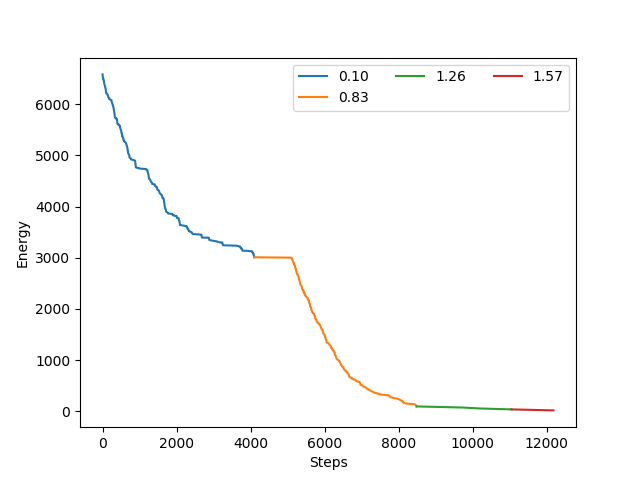
\includegraphics[width=\textwidth]{plot_energy_1000_10000.png}
        \subcaption{Energy for $\alpha=10$}
    \end{subfigure}
    \begin{subfigure}{0.49\textwidth}
        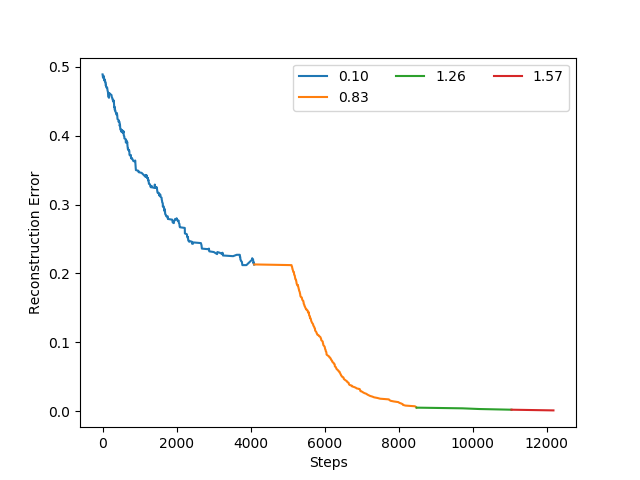
\includegraphics[width=\textwidth]{plot_error_1000_10000.png}
        \subcaption{Reconstruction Error for $\alpha=10$}
    \end{subfigure}
        \begin{subfigure}{0.49\textwidth}
        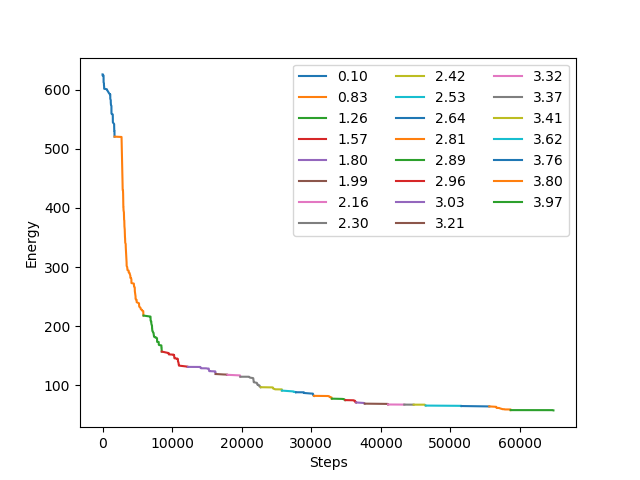
\includegraphics[width=\textwidth]{plot_energy_1000_1000.png}
        \subcaption{Energy for $\alpha=1$}
    \end{subfigure}
    \begin{subfigure}{0.49\textwidth}
        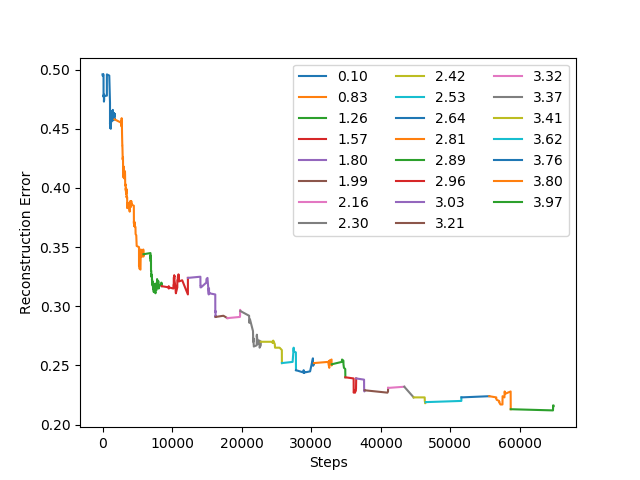
\includegraphics[width=\textwidth]{plot_error_1000_1000.png}
        \subcaption{Reconstruction Error for $\alpha=1$}
    \end{subfigure}
    \caption{Evolution of energy $H_Y$ and reconstruction error $e$ over the steps. We optimize for $n=1000$ dimensions. On the top we have have $m=10000$ observations and on the bottom $m=1000$ observations, respectively. For $\alpha=10$ we can reach the optimum of $0$ reconstruction error.}
    \label{fig:evolution}
\end{figure}

Afterwards we aim to analyze the performance of the Metropolis chain versus the Glauber dynamics variant of MCMC. For $n=1000$ and $\alpha = 1$ we run MH and the Glauber dynamics for ten runs each. We plot the energy over the steps in Figure~\ref{fig:mh_vs_glauber} on a log-scale. Both variants use the same logarithmic beta-scheduling. We can observe that the energy decreases more quickly, when using the Glauber dynamics approach in all runs. Regarding the reconstruction error the Glauber dynamics approach also seems to perform better. Note also that the MH variant stops earlier than the Glauber variant, which means that the minimal energy is less often updated and the steps counter is less frequently reset in consequence.

\begin{figure}[h]
    \centering
    \begin{subfigure}{0.49\textwidth}
        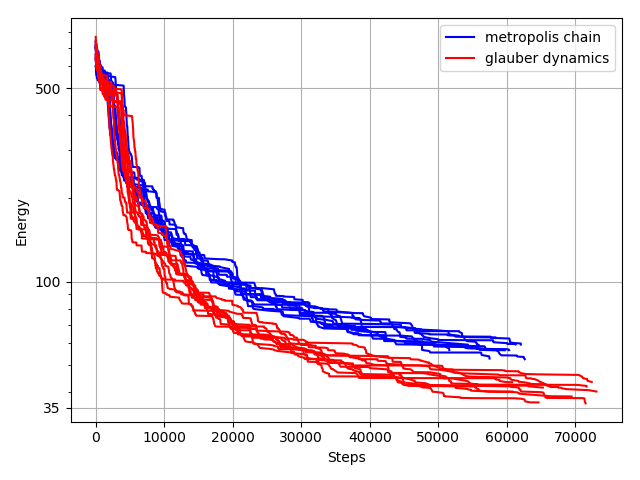
\includegraphics[width=\textwidth]{energy_comp.png}
        \subcaption{Comparison wrt. energy.}
    \end{subfigure}
    \begin{subfigure}{0.49\textwidth}
        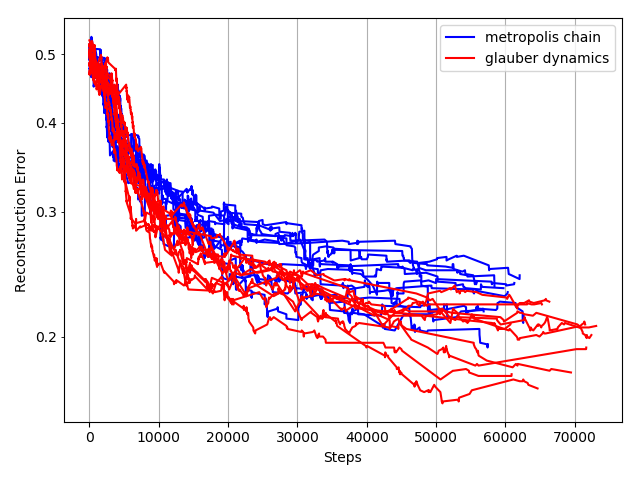
\includegraphics[width=\textwidth]{reconstruction_comp.png}
        \subcaption{Comparison wrt. reconstruction error.}
    \end{subfigure}
    \caption{Comparison of the Metropolis chain and Glauber dynamics variant of the MCMC algorithm. For each algorithm we simulated ten runs and compare the evolution of energy and reconstruction on a log-scale. We run the experiments for fixed $W$ and $Y$. The matrix dimension and observation number are set to $n=1000$ and $m=1000$, respectively. The Glauber dynamics variant shows a better performance.}
    \label{fig:mh_vs_glauber}
\end{figure}


Comparing Metropolis to Glauber we can say that the latter performs better on our problem. It is able to obtain lower energies and reconstruction errors for the same cooling schedule and number of iterations.
When plotting the result of the expected value of reconstruction error as a function of the parameter $\alpha = \frac{m}{n}$ we can observe an almost linear dependency up to a value of about 1.15, where drop tends to become steeper, taking more of a polynomial form (Figure~\ref{fig:alpha_both}). We can therefore name $\alpha_c = 1.15$ to be the critical value.
Also we observe an $\alpha_{rdm}$ with a value at around 0.01. For $\alpha < \alpha_{rdm}$ we observe a reconstruction error of about 0.5, which is characteristic for a pure random guess. The expected value of the error does not go above 0.5, as our estimation is still better informed than a random guess.
For larger values of $\alpha$ we always get an optimal result with zero reconstruction error.

\begin{figure}[h]
    \centering
    \begin{subfigure}{0.49\textwidth}
        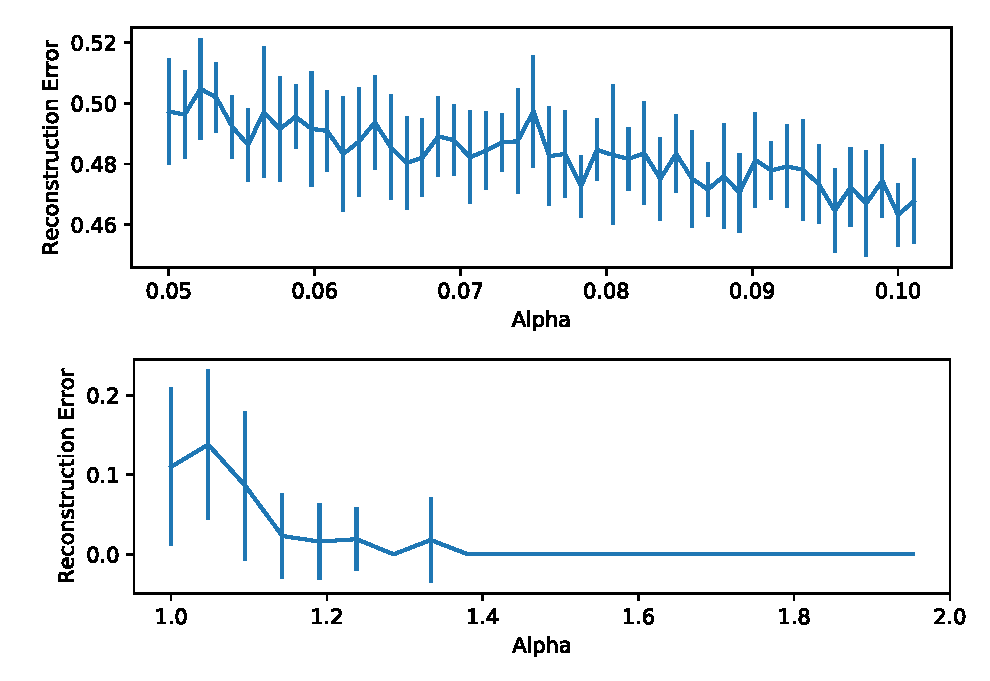
\includegraphics[width=\textwidth]{critical_values.pdf}
    \end{subfigure}
    \begin{subfigure}{0.49\textwidth}
    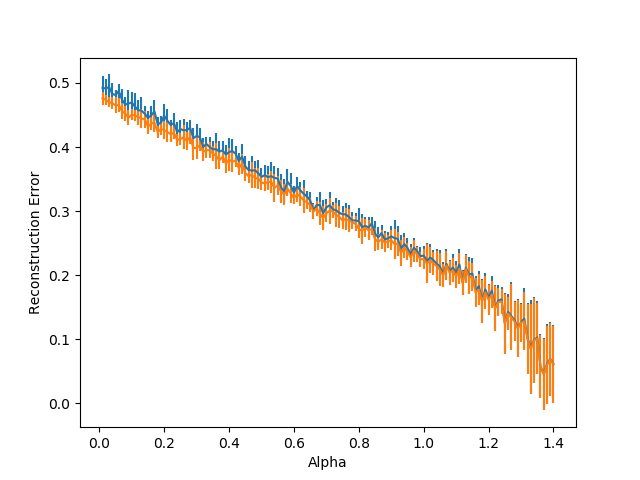
\includegraphics[height=6cm]{alpha_both.png}
    \end{subfigure}
    \caption{Expected value and variance of the reconstruction error for different settings of $\alpha = \frac{m}{n}$} Blue: last estimation for each alpha. Orange: lowest error estimation
    \label{fig:alpha_both}
\end{figure}


\begin{thebibliography}{9}

\bibitem{1}
  Mathias Ortner, Xavier Descombes, Josiane Zerubia,
  \textit{An adaptive simulated annealing cooling schedule for object detection in images},
  RR-6336,
  2007.

\end{thebibliography}
\end{document}
